\documentclass{article}

\usepackage[preprint]{neurips_2026}

\usepackage[utf8]{inputenc}
\usepackage[T1]{fontenc}
\renewcommand{\ttdefault}{lmtt}
\usepackage{hyperref}
\usepackage{url}
\usepackage{booktabs}
\usepackage{amsfonts}
\usepackage{amsmath}
\usepackage{nicefrac}
\usepackage{microtype}
\usepackage{xcolor}
\usepackage{graphicx}
\usepackage{subcaption}

\graphicspath{{../figures/}}
\newcommand{\growE}{\textsc{Grow-early}}
\newcommand{\growL}{\textsc{Grow-late}}

\hypersetup{colorlinks=true, linkcolor=blue!50!black, citecolor=blue!50!black, urlcolor=blue!50!black}

\title{Grow Instead of Search? Function-Preserving Depth Growth for Multi-Task PPO on Meta-World MT10}

\author{%
  COMP9501 Advanced Machine Learning \\
  Course project report \\
}

\begin{document}

\maketitle

\begin{abstract}
The depth of a policy network is usually chosen by training one network per candidate depth and keeping the best, which multiplies the cost of already expensive reinforcement-learning runs.
We ask whether a single run that starts shallow and grows deeper can replace this search.
New layers are inserted with an identity initialisation placed after a ReLU, which leaves the policy exactly unchanged at insertion while keeping the optimiser state of existing weights.
On Meta-World MT10 with a multi-task PPO learner, we sweep actor depths 1--4 and compare two fixed growth schedules against grid search, successive halving, a default depth and a random depth, using 43 runs of 3M environment steps each and held-out goal configurations for evaluation.
Depth matters on this benchmark (64\% to 88\% held-out success from one to four hidden layers), while held-out goals turn out to be no harder than training goals.
Growing early (depth 1$\to$3 at 0.5M and 1M steps) reaches 84\% held-out success for the cost of one run, comparable to simulated successive halving (85\%) at 55\% of its environment steps and about half of its learner FLOPs, and 4.8 points better than committing to a random depth.
It remains 5.0 points below the best fixed depth, growing late is no better than a random depth, and with a narrow actor growth does not help.
Measured GPU time does not separate the methods at this model size, so we report environment steps and FLOPs.
\end{abstract}

\section{Introduction}

Network size is one of the few hyperparameters that is rarely tuned per problem in deep reinforcement learning (RL), even though recent work shows that it matters a great deal when the network is designed to scale \citep{nauman2024bro,lee2025simba}.
The standard way to choose it is search: train one agent per candidate architecture and keep the one that does best on validation.
In RL each training run consumes millions of simulator interactions, so a search over $K$ depths multiplies an already large cost by $K$, and results are notoriously sensitive to seeds \citep{henderson2018matters}.

Function-preserving growth \citep{chen2016net2net} suggests an alternative: start with a small network and add layers during training, initialised so that the function computed by the network does not change.
If growth reached the performance of the best depth, one run would replace $K$.
For RL this is not obvious.
A new layer starts with fresh optimiser statistics and must become useful while the policy is collecting its own data, and networks in RL are known to lose plasticity as training proceeds \citep{nikishin2022primacy,lyle2023plasticity}.
The time at which a layer is added may therefore matter as much as whether it is added.

We study this question in a controlled setting: a multi-task PPO learner \citep{schulman2017ppo,li2026toppo} on Meta-World MT10 \citep{yu2020metaworld}, with only the depth of the actor varied.
Our problem framing is explicit about cost: \emph{the right depth is not known in advance, and the cost of any method includes every environment step spent before a final model is chosen}.
Under this framing, a fixed depth is not a free baseline; it is a guess.
Our contributions are:
\begin{itemize}
    \item A reproducible protocol and runner for depth sweeps and scheduled growth on MT10 with separate train, validation and held-out test goals per task, logging success on all three every 0.5M steps (43 runs, 5 seeds at width 400).
    \item Evidence that identity insertion after a ReLU adds depth with zero change to the policy, and that growing runs show no performance dip at insertion.
    \item A cost-aware comparison showing that growing early matches simulated successive halving at 55\% of its environment steps but stays below the best fixed depth, and that the benefit depends on the growth schedule and on width.
\end{itemize}

\section{Related work}

\paragraph{Growing networks.}
Net2Net \citep{chen2016net2net} introduced function-preserving widening and deepening, using identity initialisation for new layers.
Later methods choose where and how to grow from gradient information \citep{evci2022gradmax,wu2020firefly}, and progressive stacking reduces the cost of training large language models by copying layers \citep{gong2019stacking}.
These works mostly target supervised learning, where the data distribution does not change when the network grows.

\paragraph{Hyperparameter search under a budget.}
Successive halving and Hyperband \citep{jamieson2016sh,li2018hyperband} allocate more budget to promising configurations and stop poor ones early; population-based training \citep{jaderberg2017pbt} adapts hyperparameters within a population.
We use successive halving as the strongest cheap search baseline, since it uses the same learning curves as grid search but discards most of the cost.

\paragraph{Network scale in RL.}
Larger networks help in continuous control when combined with normalisation and regularisation \citep{nauman2024bro,lee2025simba}, while training dynamics in RL can reduce a network's ability to keep learning \citep{nikishin2022primacy,lyle2023plasticity}.
Our learner normalises per-task value targets with PopArt \citep{vanhasselt2016popart,hessel2019popart} and uses a LayerNorm critic \citep{ba2016layernorm}, following the reference implementation \citep{li2026toppo}.

\section{Method}

\paragraph{Identity insertion.}
Let the actor body end with a hidden representation $h = \mathrm{ReLU}(z) \in \mathbb{R}_{\ge 0}^{W}$.
We append a bias-free linear layer $W_{\text{new}} \in \mathbb{R}^{W\times W}$ followed by a ReLU, initialised to $W_{\text{new}} = I$.
Because $h \ge 0$ element-wise,
\begin{equation}
    \mathrm{ReLU}(W_{\text{new}}\, h) = \mathrm{ReLU}(h) = h ,
\end{equation}
so the action mean, the state-independent action standard deviation and therefore the whole Gaussian policy are unchanged at insertion.
The critic is not modified.
All existing parameters keep their Adam \citep{kingma2015adam} moment estimates; the new layer is added as a new parameter group with the same learning rate and fresh moments, and is included in gradient clipping.
Our implementation asserts that the action mean changes by at most $10^{-5}$ on probe observations, that the action standard deviation and critic output are bit-identical, and that the optimiser state of existing parameters and the global random-number state are unchanged.
Each insertion at width 400 adds 160{,}000 actor parameters.

\paragraph{Growth schedules.}
All growth runs start at depth 1 and insert two layers, ending at depth 3:
\growE{} inserts at 0.5M and 1M environment steps, \growL{} at 1M and 2M.
Insertions happen only between PPO iterations, when the rollout buffer is empty.

\section{Experimental setup}

\paragraph{Environment and learner.}
We use Meta-World MT10 \citep{yu2020metaworld} (MuJoCo \citep{todorov2012mujoco}): ten manipulation tasks learned by one policy conditioned on a one-hot task identifier.
The learner is the multi-task PPO of \citet{li2026toppo} with GAE \citep{schulman2016gae} ($\lambda = 0.97$, $\gamma = 0.99$), clip range 0.2, value clipping, entropy coefficient 0.005, learning rate $3\times10^{-4}$, 100k-step rollouts from 10 parallel environments, 16 epochs per rollout with stratified mini-batches of 3{,}125, PopArt value normalisation and a 3-layer, width-400 LayerNorm critic (342k parameters).
Only the actor's hidden depth (1--4 layers of width 400; a secondary study uses width 128) or its growth schedule differs between runs.
Every run gets 3M environment steps.

\paragraph{Goal split and evaluation.}
Each MT10 task has 50 goal configurations (object and target positions).
With a fixed benchmark seed we use goals 0--29 for training, 30--39 for validation and model selection, and 40--49 as held-out test goals (Figure~\ref{fig:goals}).
Every 0.5M steps we run one episode with the evaluation-mode policy on 10 training, 10 validation and 10 test goals for each task (300 episodes); success is Meta-World's binary success signal at any step of the episode.
All numbers reported are held-out test success unless stated otherwise.

\begin{figure}[t]
    \centering
    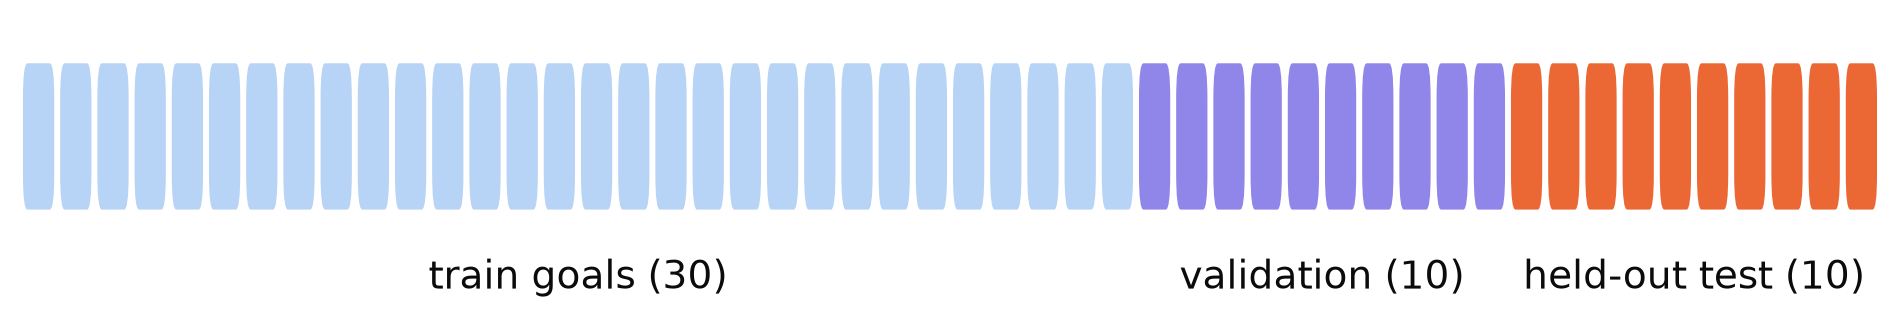
\includegraphics[width=0.85\linewidth]{static/goal_split.png}
    \caption{Per-task split of the 50 MT10 goal configurations.}
    \label{fig:goals}
\end{figure}

\paragraph{Baselines and cost accounting.}
We compare strategies for producing one final policy when the depth is unknown, with $K=4$ candidate depths and $T=3$M steps per run:
\emph{grid search} trains all four depths and selects by final validation success (cost $4T$);
\emph{successive halving} \citep{jamieson2016sh} trains all four depths to $T/6$, keeps the best two by validation success until $T/2$ and the best one until $T$ (cost $5.5$M steps).
It is simulated from the logged validation curves of the same runs, so it uses no extra training and gets exactly the learning curves grid search sees.
\emph{Default depth 2} is the reference recipe's depth; \emph{random depth} is the mean over the four depths, the expected outcome of guessing;
\emph{best depth in hindsight} picks the depth with the highest test success per seed and is an upper reference rather than an achievable method.
Comparisons are paired by seed: for a given seed, every strategy is evaluated on the runs with that seed.

We report two costs.
Environment steps count every training interaction.
Learner compute counts the floating-point operations of the actor and critic: per training sample, $2P$ for the rollout forward pass and $16\times 6P$ for the 16 PPO epochs, where $P$ is the number of actor plus critic parameters at that time.
We also logged synchronised GPU time of policy inference and PPO updates.

\paragraph{Compute.}
Runs were distributed over an 8$\times$RTX A6000 server, Modal T4 instances, an RTX 4070 and an RTX 3050; a 3M-step run took 34--65 minutes of wall-clock time.
Because hardware differed between runs, GPU-time comparisons use only A6000 runs.

\section{Results}

\begin{figure}[t]
    \centering
    \begin{subfigure}[t]{0.49\linewidth}
        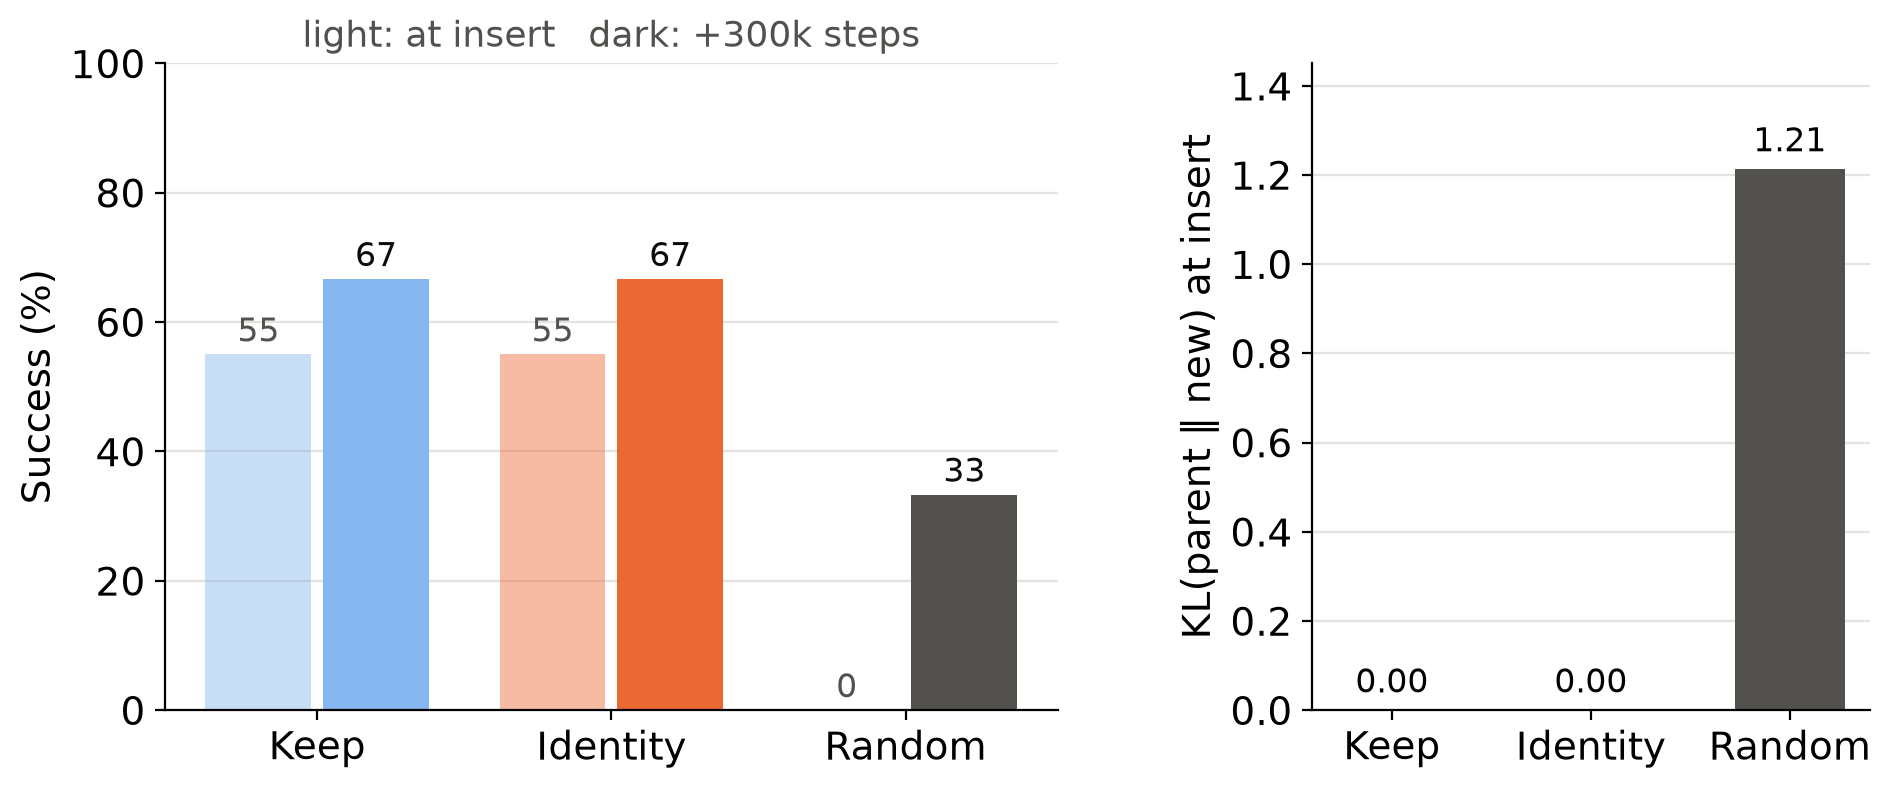
\includegraphics[width=\linewidth]{static/pilot_insertion.png}
        \caption{Pilot insertion test}
        \label{fig:pilot}
    \end{subfigure}\hfill
    \begin{subfigure}[t]{0.49\linewidth}
        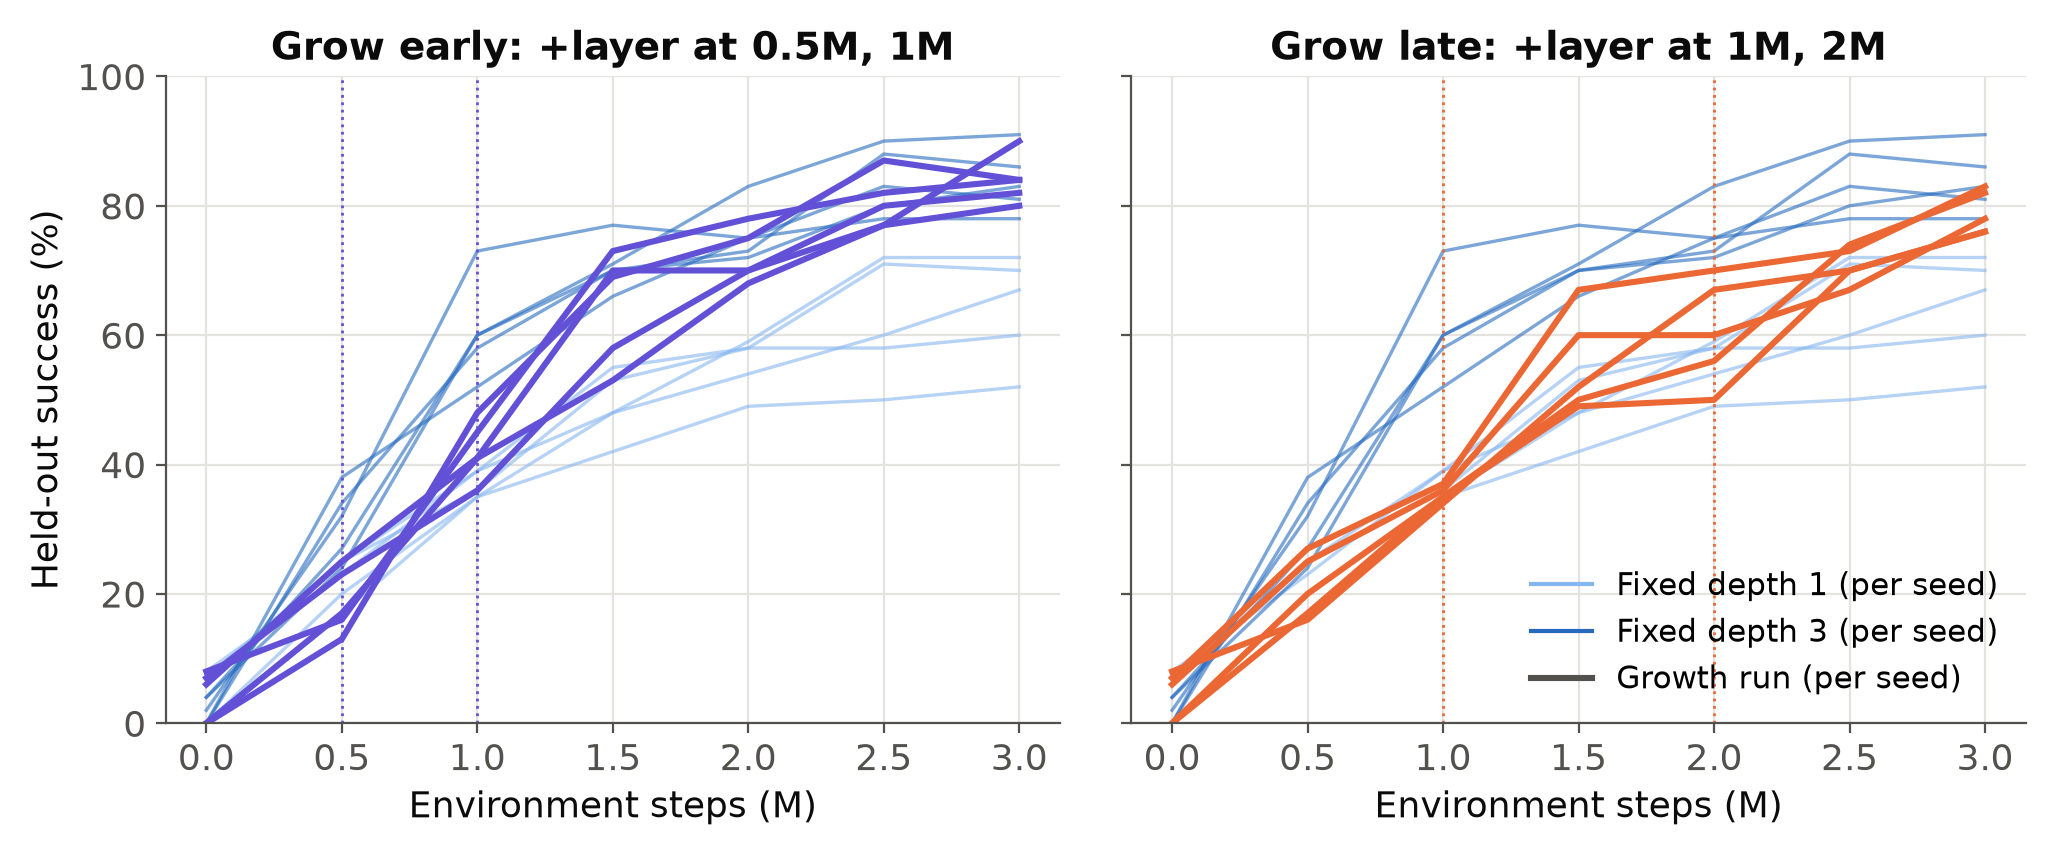
\includegraphics[width=\linewidth]{w400/growth_traj.png}
        \caption{Growth trajectories}
        \label{fig:traj}
    \end{subfigure}
    \caption{(a) Pilot on three MT10 tasks (one seed, 60 held-out episodes): success at insertion (light) and 300k steps later (dark), and KL divergence between the parent policy and the new policy at insertion. (b) Held-out success of each growth run (bold) against fixed depth 1 and depth 3 runs of all seeds; dotted lines mark insertions.}
    \label{fig:insert}
\end{figure}

\paragraph{Identity insertion does not disturb the policy.}
In a pilot on three tasks (Figure~\ref{fig:pilot}), inserting an identity layer into a trained parent left the policy unchanged (KL $= 0$, 33/60 successes at insertion, as without insertion), and the grown policy continued to learn exactly as well as the unchanged one over the next 300k steps.
A randomly initialised layer instead produced KL $= 1.21$ and zero success at insertion, recovering only to 20/60.
In the main study all 20 insertions (10 growth runs, two each) had a maximum action-mean error of 0, and no growth run shows a drop in held-out success after an insertion (Figure~\ref{fig:traj}).

\begin{figure}[t]
    \centering
    \begin{subfigure}[t]{0.49\linewidth}
        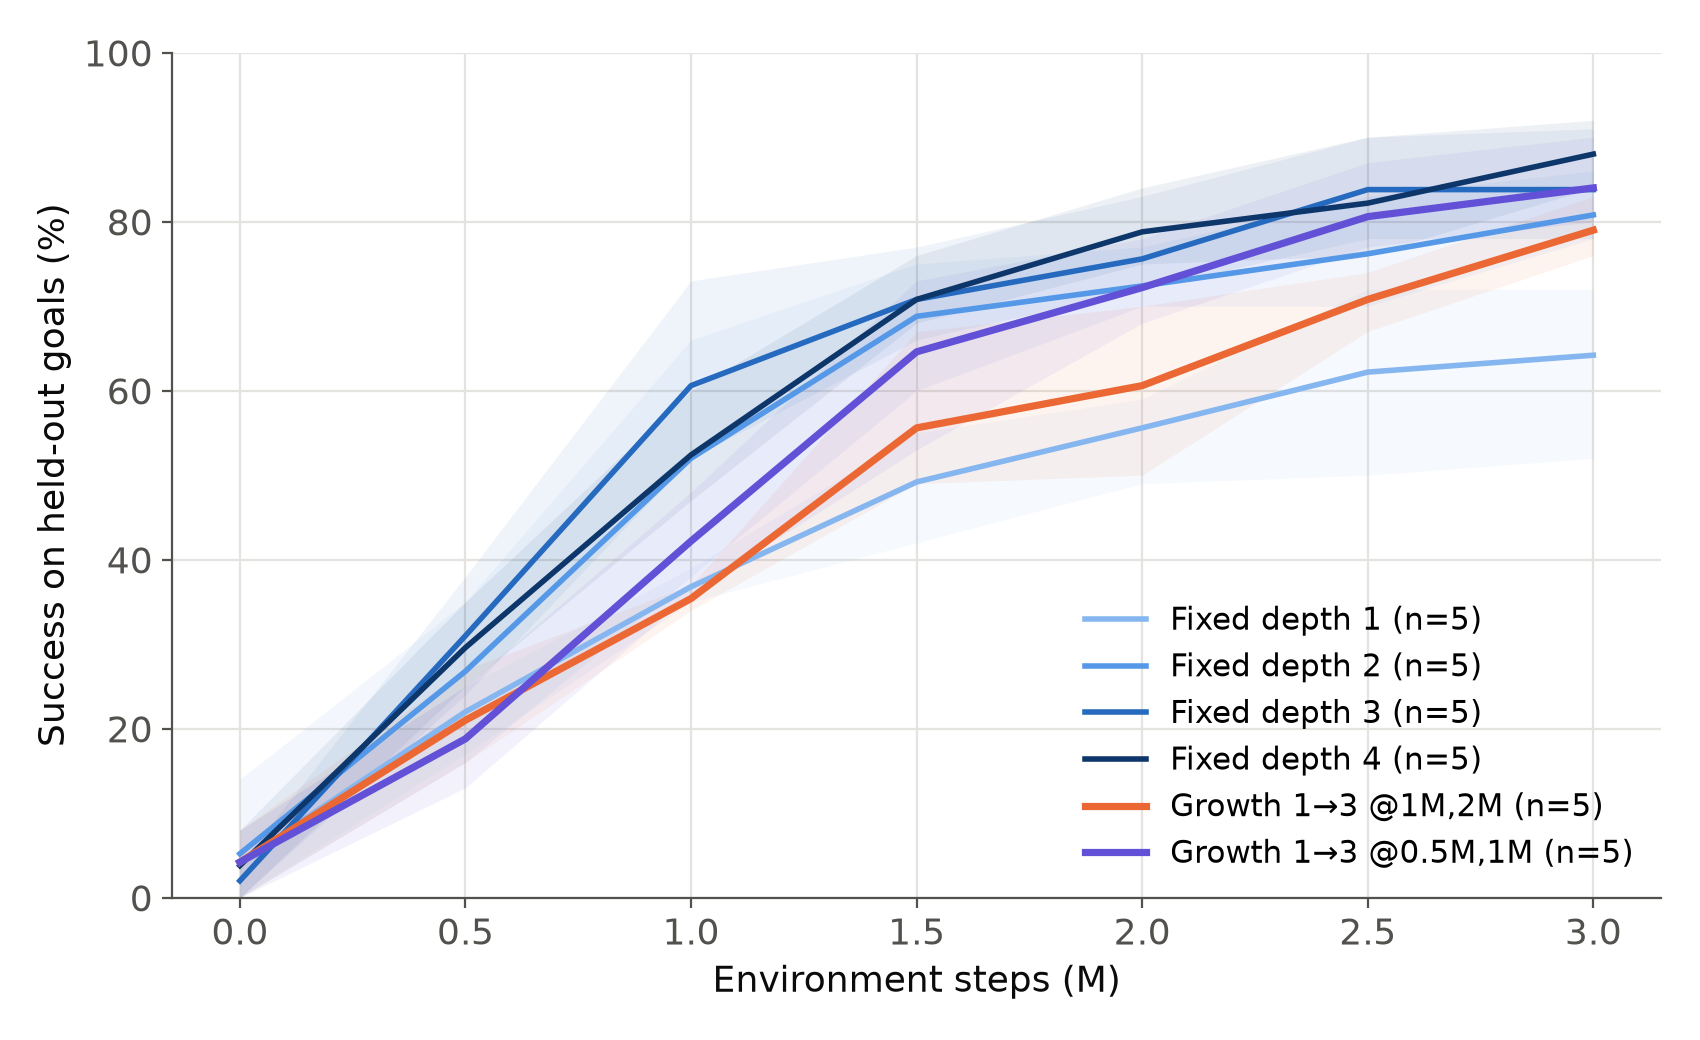
\includegraphics[width=\linewidth]{w400/curves_success_test.png}
        \caption{Held-out success during training}
        \label{fig:curves}
    \end{subfigure}\hfill
    \begin{subfigure}[t]{0.49\linewidth}
        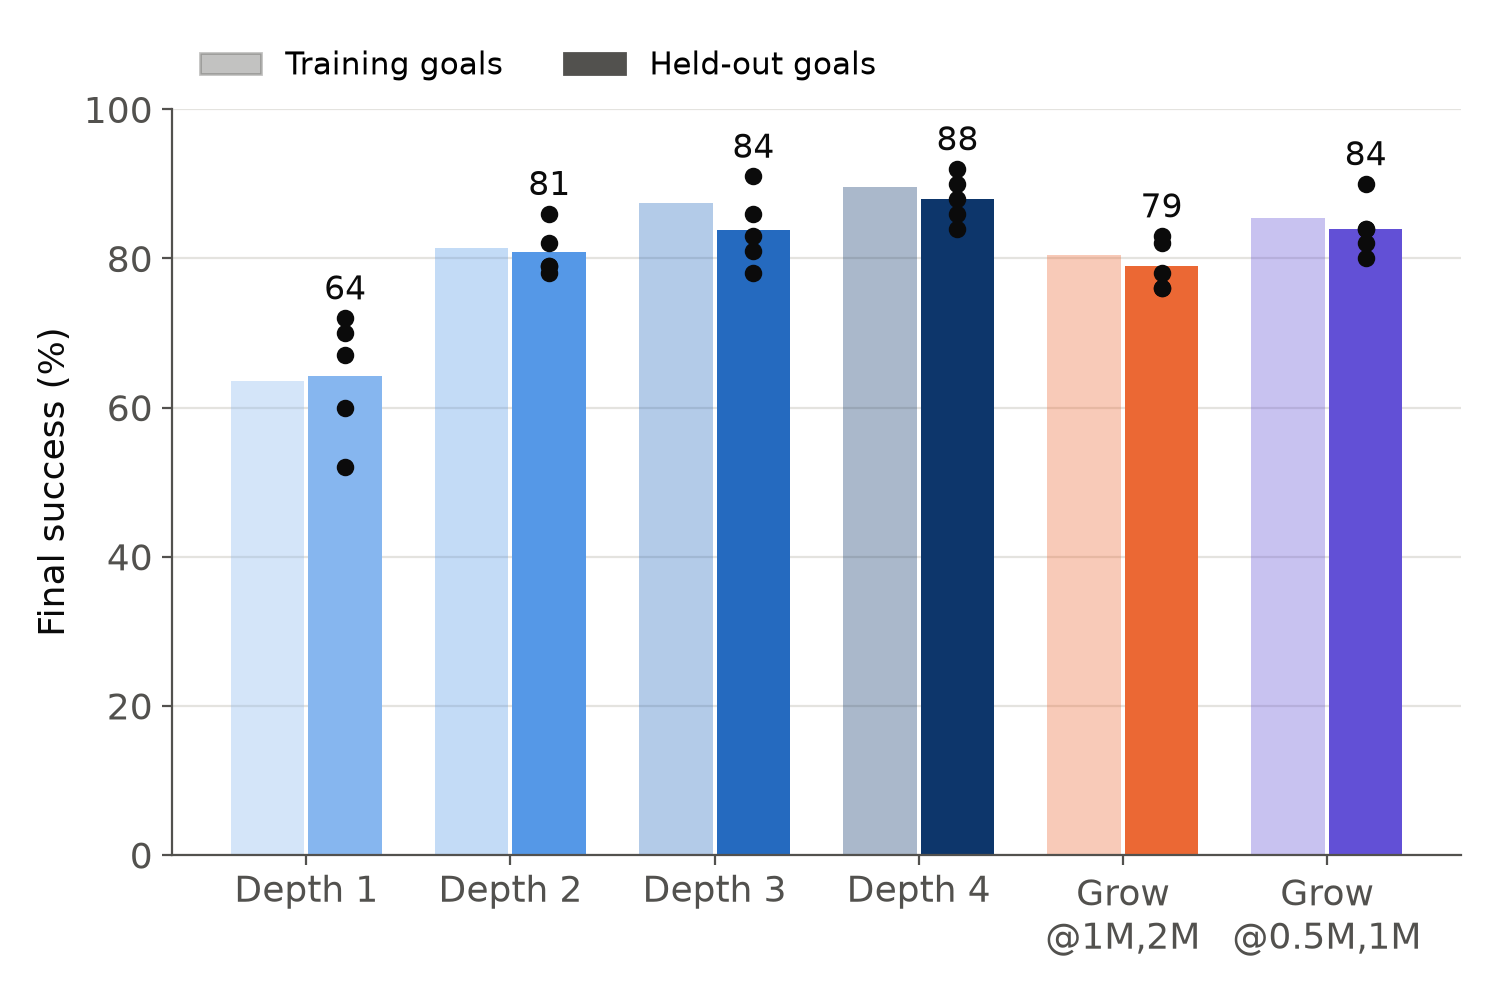
\includegraphics[width=\linewidth]{w400/final_by_depth.png}
        \caption{Final success, training vs held-out goals}
        \label{fig:final}
    \end{subfigure}
    \caption{Width 400, five seeds. (a) Mean and range over seeds. (b) Light bars: training goals; dark bars: held-out goals; dots: individual seeds.}
    \label{fig:depth}
\end{figure}

\paragraph{Held-out goals are not harder than training goals.}
Across all six configurations, final success on training goals exceeds held-out success by between $-0.6$ and $3.6$ points (Figure~\ref{fig:final}).
The goal configurations of a task interpolate one another, so the split is a valid held-out test but does not make MT10 noticeably harder.
Earlier internal experiments that reported above 90\% success on training goals were therefore not mainly measuring memorisation of goal positions.

\paragraph{Depth matters.}
Final held-out success rises from 64\% (depth 1) to 81\%, 84\% and 88\% for depths 2--4 (Figure~\ref{fig:curves}, Table~\ref{tab:main}).
Deeper actors also learn faster after about 0.7M steps.
The best depth in hindsight is 3 for two seeds and 4 for three, and validation selects the same depth as test selection in all five seeds.
Per task (Figure~\ref{fig:pertask}), six tasks are solved at every depth; the gains come from \texttt{peg-insert-side} (0\% $\to$ 76\%), \texttt{push} (22\% $\to$ 88\%) and \texttt{drawer-open} (40\% $\to$ 100\%), while \texttt{pick-place} stays below 20\% for every configuration within this budget.

\begin{figure}[t]
    \centering
    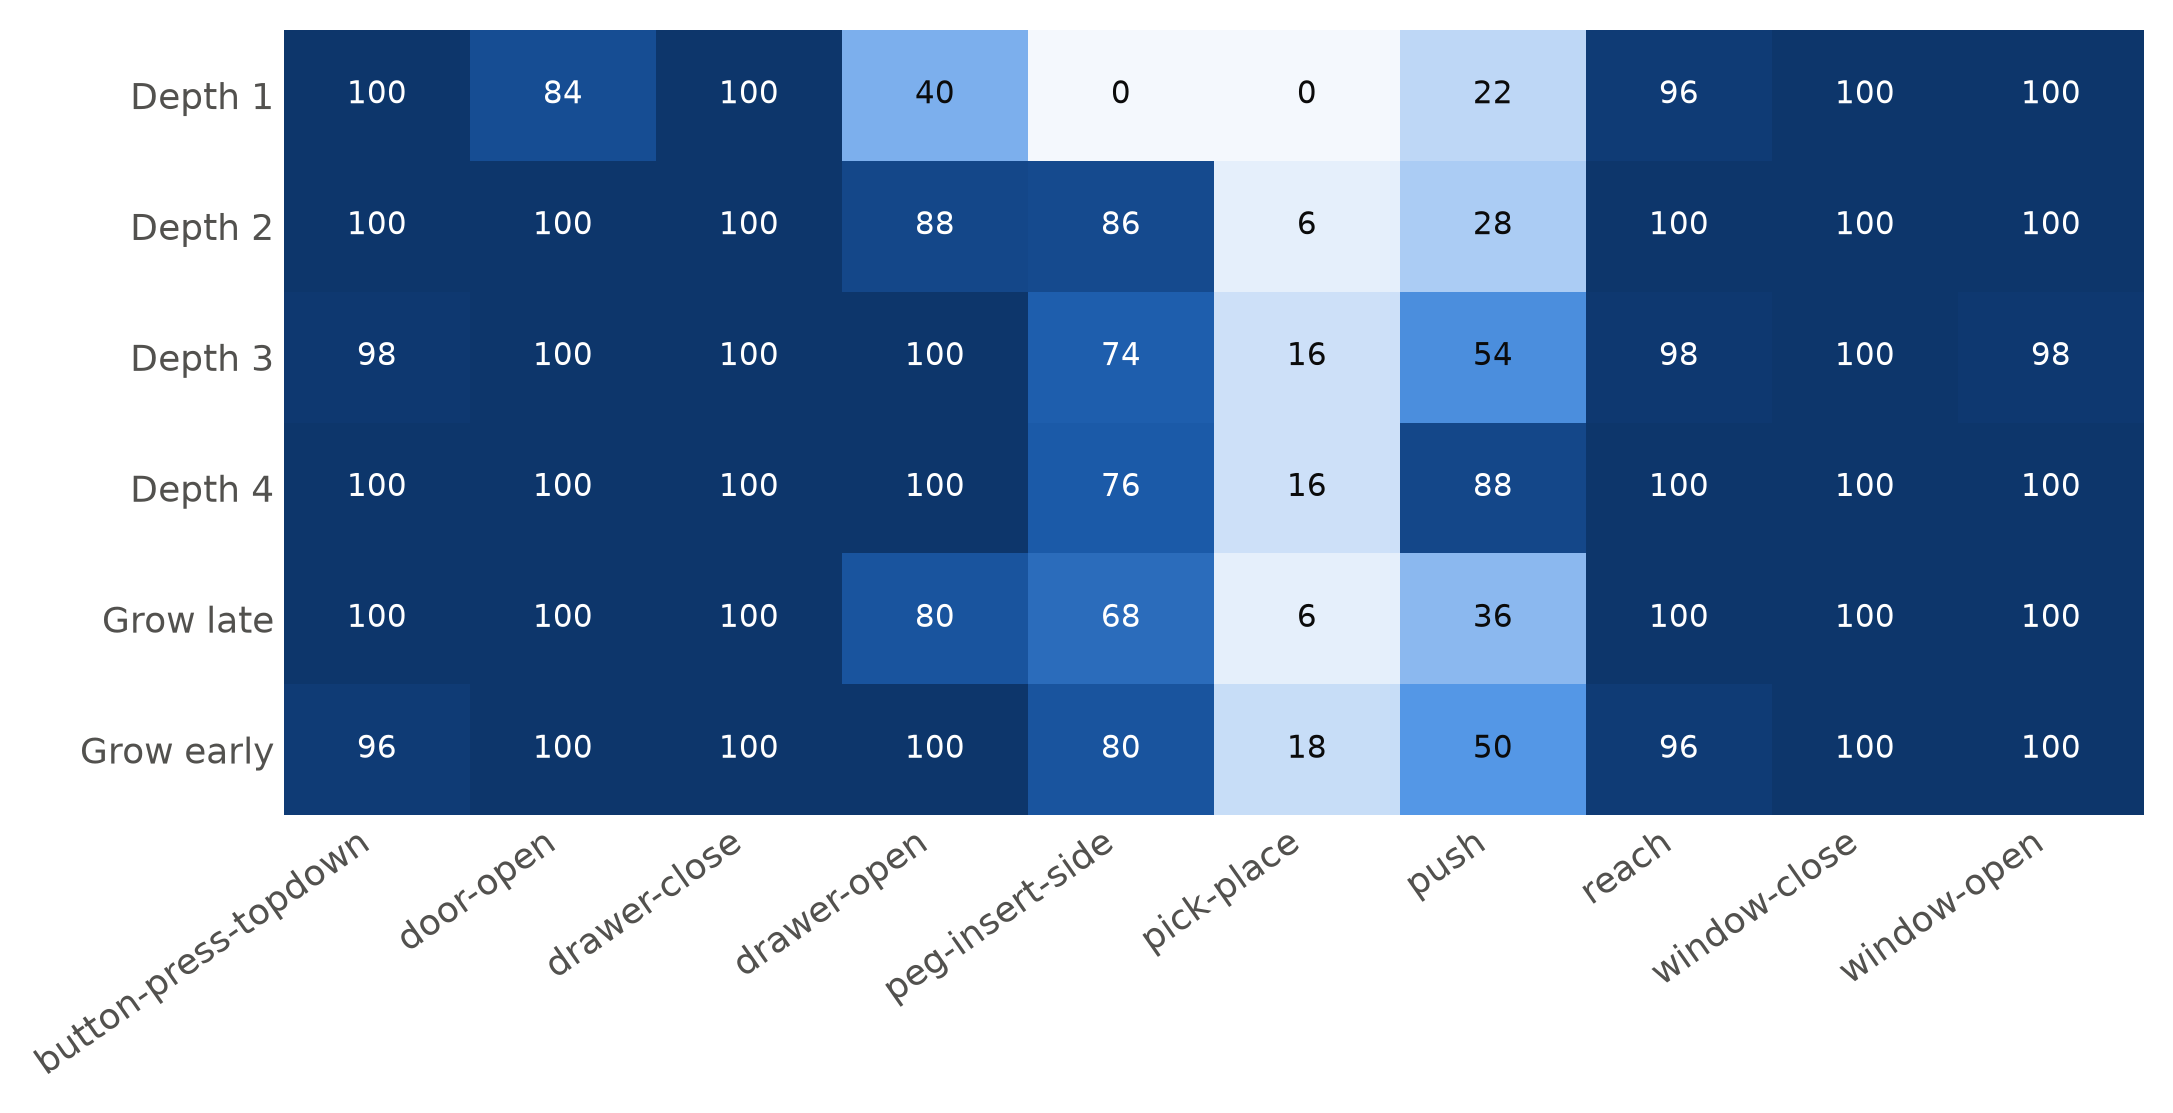
\includegraphics[width=0.9\linewidth]{w400/per_task.png}
    \caption{Final held-out success per task (\%), mean over five seeds, width 400.}
    \label{fig:pertask}
\end{figure}

\paragraph{Growing early matches cheap search; growing late does not.}
Table~\ref{tab:main} and Figure~\ref{fig:strategy} compare the strategies.
\growE{} reaches 84.0\% with a single 3M-step run.
This is close to successive halving (85.2\%, 5.5M steps) and 3.2 and 4.8 points above the default depth and a random depth.
It is 5.0 points below the best fixed depth, which grid search also finds, at four times the cost.
Paired over seeds, the advantage of \growE{} over a random depth ($+4.8 \pm 3.6$, 95\% interval) and over \growL{} ($+5.0 \pm 3.0$) and its gap to the best depth ($-5.0 \pm 3.7$) are larger than the seed-to-seed variation, whereas its differences from successive halving ($-1.2 \pm 8.2$) and from default depth 2 ($+3.2 \pm 6.8$) are not resolved with five seeds.
The trajectories in Figure~\ref{fig:traj} explain the role of timing: \growE{} spends 2M steps at depth 3 and joins the fixed deep networks, while \growL{} spends only 1M steps at depth 3 and ends at the level of depth 2.
Per task, \growE{} recovers \texttt{drawer-open} and \texttt{peg-insert-side} but reaches only 50\% on \texttt{push}, where depth 4 reaches 88\%.

\begin{table}[t]
    \caption{Strategies for producing one policy without knowing the right depth (width 400, five paired seeds). Success is held-out test success at 3M steps of the chosen run (mean $\pm$ standard error). Costs include all runs a strategy trains. $^\dagger$Requires knowing test results; not achievable without search.}
    \label{tab:main}
    \centering
    \begin{tabular}{lccc}
        \toprule
        Strategy & Success (\%) & Env.\ steps (M) & Learner PFLOP \\
        \midrule
        Grid search, depths 1--4      & $89.0 \pm 1.3$ & 12.0 & 0.71 \\
        Successive halving (simulated) & $85.2 \pm 2.9$ & 5.5  & 0.36 \\
        Default depth 2                & $80.8 \pm 1.5$ & 3.0  & 0.15 \\
        Random depth (mean of 1--4)    & $79.2 \pm 1.1$ & 3.0  & 0.18 \\
        \growL{} (1$\to$3 at 1M, 2M)   & $79.0 \pm 1.5$ & 3.0  & 0.15 \\
        \growE{} (1$\to$3 at 0.5M, 1M) & $84.0 \pm 1.7$ & 3.0  & 0.18 \\
        \midrule
        Best fixed depth$^\dagger$     & $89.0 \pm 1.3$ & 3.0  & 0.23 \\
        \bottomrule
    \end{tabular}
\end{table}

\begin{figure}[t]
    \centering
    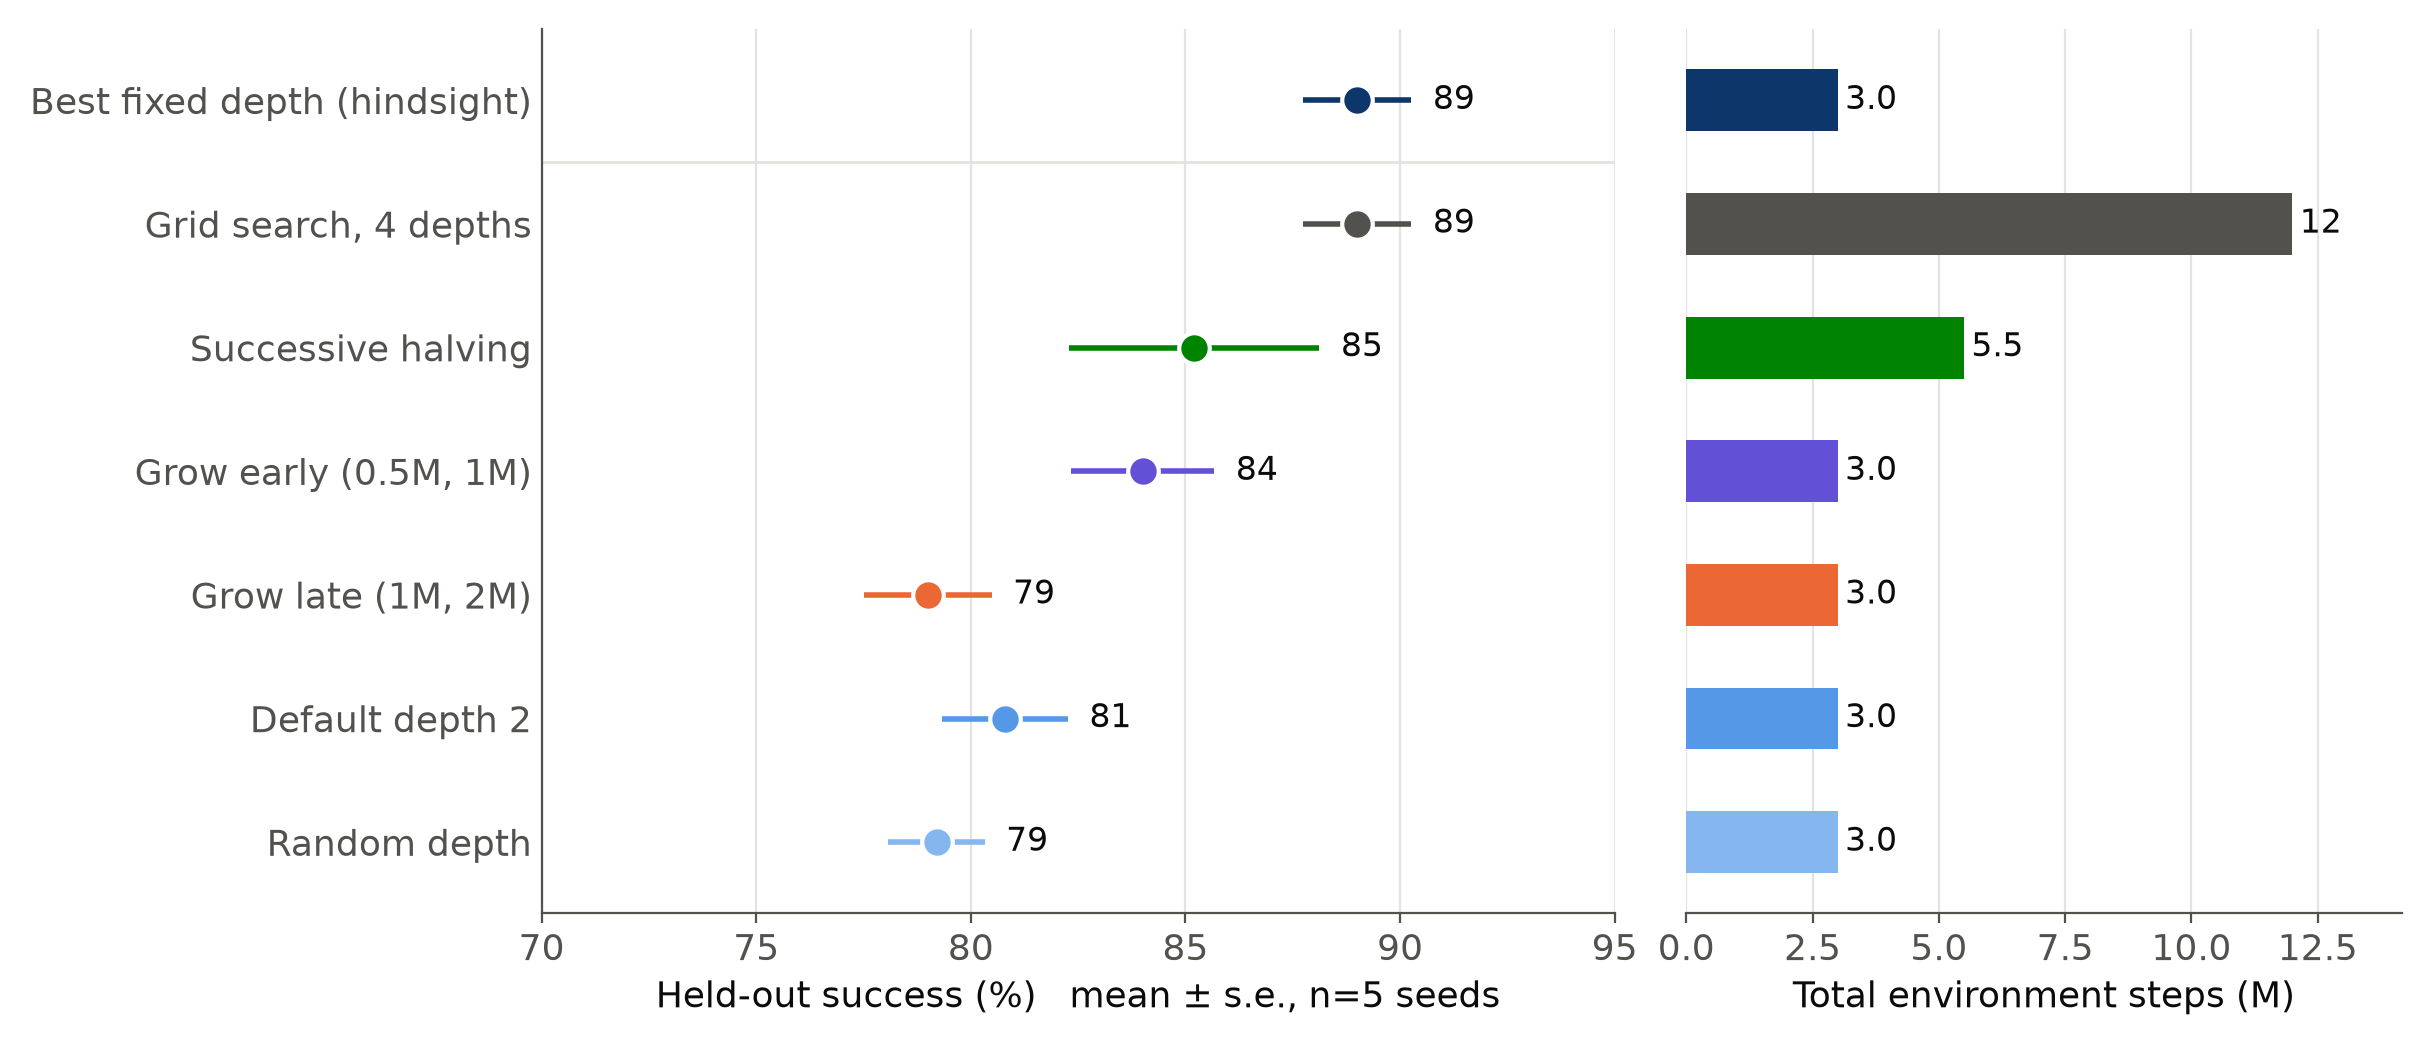
\includegraphics[width=\linewidth]{w400/strategy_panel.png}
    \caption{Held-out success (left, mean $\pm$ s.e.\ over five paired seeds) and total environment steps (right) of each strategy at width 400.}
    \label{fig:strategy}
\end{figure}

\paragraph{Compute and GPU time.}
In learner FLOPs, \growE{} costs 0.18 PFLOP, a quarter of grid search (0.71), half of successive halving (0.36), and less than training depth 4 directly (0.25), because it spends its first 1M steps in smaller networks (Figure~\ref{fig:compute}).
Measured GPU time, which we had hoped to use as the cost axis, does not reflect this: on A6000 runs it ranges from 10 to 17 minutes per run with no consistent trend over depth, although FLOPs grow 2.3$\times$ from depth 1 to depth 4.
With a few hundred thousand parameters, each forward and backward pass is dominated by kernel-launch and synchronisation overhead, and run-to-run variation came mostly from load on the shared server.
GPU time is therefore not a useful cost measure at this scale; wall-clock time is dominated by CPU simulation in any case (a full run took 34--65 minutes, of which GPU work was roughly a quarter).

\begin{figure}[t]
    \centering
    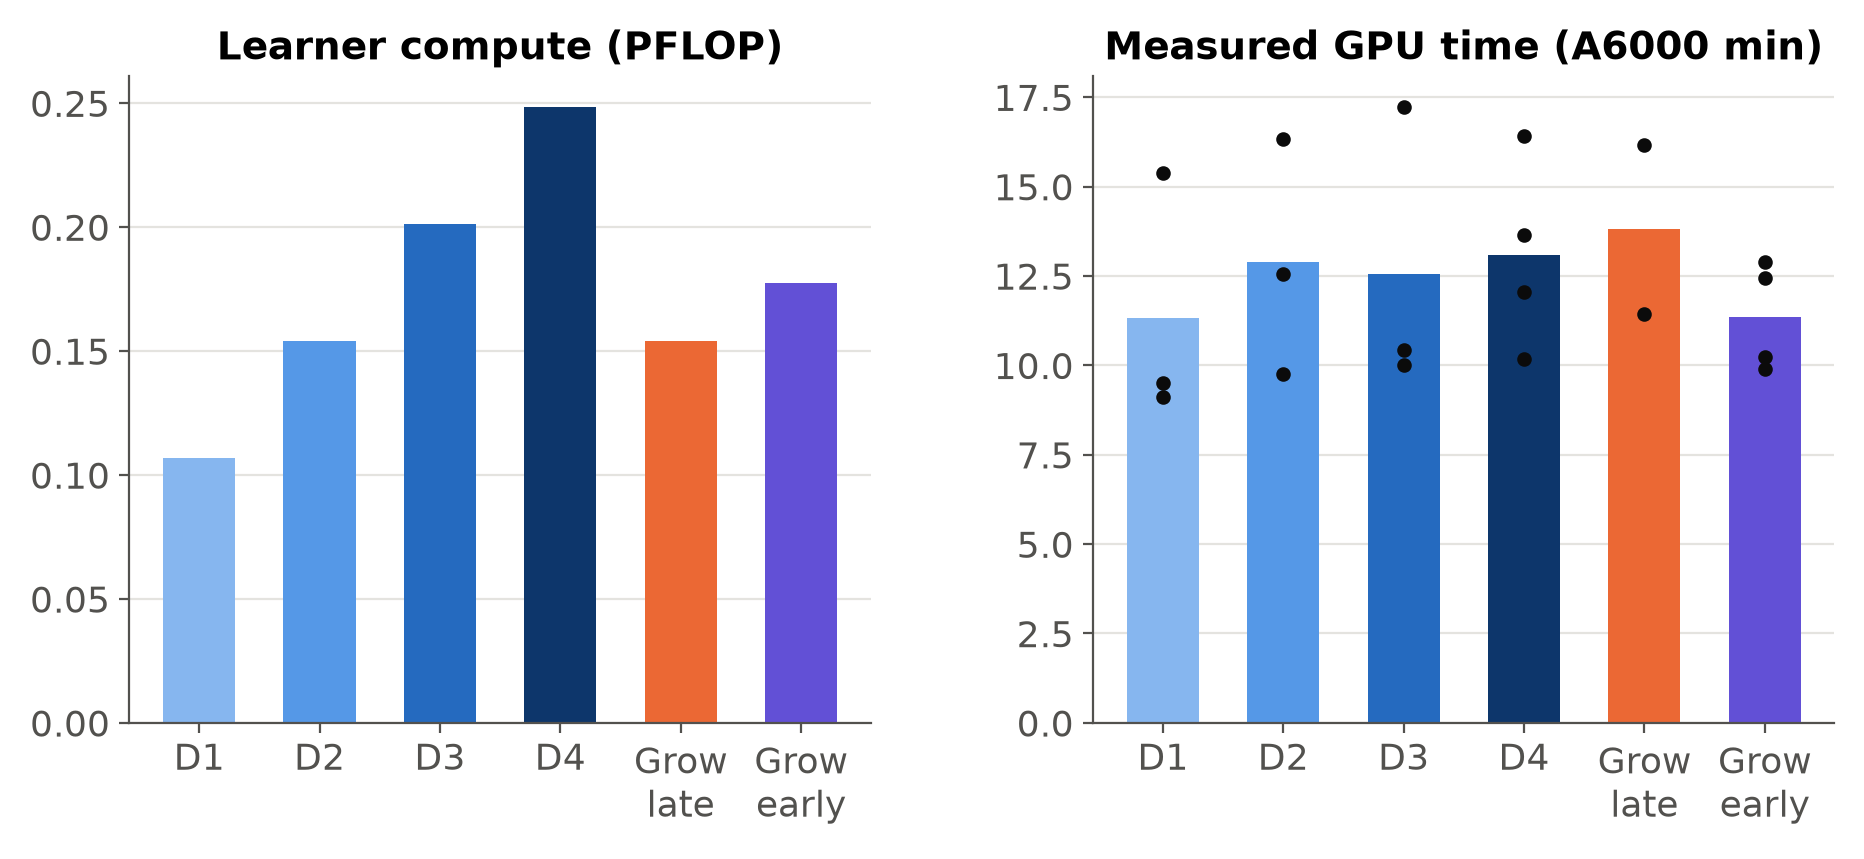
\includegraphics[width=0.85\linewidth]{w400/compute_vs_gpu.png}
    \caption{Learner compute per run (left) and measured GPU time per run on A6000 GPUs (right, dots are individual runs), width 400.}
    \label{fig:compute}
\end{figure}

\paragraph{With a narrow actor, growth does not help.}
At width 128 (two seeds; Figure~\ref{fig:w128} in the appendix), the best fixed depth reaches 82\% and successive halving 80\%, but \growE{} reaches only 71\% and \growL{} 66\%, both below a random depth (72\%).
Two seeds are too few for a conclusion, but the result warns that the benefit of growth is not automatic: a narrow layer that starts as the identity and has fresh optimiser state may not become useful within the remaining budget.

\section{Discussion and limitations}

\paragraph{What the results support.}
When the right depth is unknown, growing early is a reasonable default: it costs one run, avoids an insertion shock and performs like successive halving on this benchmark.
It does not replace a full search when the last few points matter; the best fixed depth is still 5 points better.
The timing result suggests that the useful quantity is time spent at the final depth, consistent with the view that capacity added late in RL training is harder to use \citep{nikishin2022primacy,lyle2023plasticity}.

\paragraph{Limitations.}
This is an exploratory study.
It uses one benchmark, one algorithm and five seeds (two at width 128), within a 3M-step budget; longer training could change the ranking of depths and schedules.
Growth follows fixed schedules rather than an adaptive trigger, grows only to depth 3 although depth 4 was best for three of five seeds, and only the actor grows.
Successive halving is simulated from logged curves; a real implementation would see the same curves, but its rung schedule was not tuned.
Each evaluation uses 100 held-out episodes per run, so per-run estimates carry roughly $\pm 4$ points of binomial noise, and we follow paired comparisons and interval estimates rather than single numbers \citep{agarwal2021precipice}.
Held-out goals test interpolation within tasks, not generalisation to new tasks.
Finally, runs were spread over four GPU types; environment steps and FLOPs are hardware-independent, but GPU time is compared only within A6000 runs.

\paragraph{Next steps.}
The most direct extensions are growth triggered by a plateau in validation success, growing to the depth a search would select (four layers here), growing the critic, and repeating the study on MT50, where interference between tasks may make capacity more important.

\section{Conclusion}

Function-preserving identity insertion lets a multi-task PPO policy grow deeper without any change at insertion.
On Meta-World MT10, where depth is worth up to 24 points of held-out success, growing early gives one run the performance of successive halving at 55\% of its environment steps, but not the performance of the best depth, and growing late or growing a narrow network gives no benefit.
Under a cost model that counts the search, growth is a cheap, safe default rather than a replacement for search.

\bibliographystyle{plainnat}
\bibliography{refs}

\appendix

\section{Additional results}

\begin{table}[h]
    \caption{Final held-out success (\%) of every width-400 run, by seed.}
    \label{tab:seeds}
    \centering
    \begin{tabular}{lcccccc}
        \toprule
        Seed & Depth 1 & Depth 2 & Depth 3 & Depth 4 & \growL{} & \growE{} \\
        \midrule
        1 & 60 & 86 & 91 & 88 & 78 & 82 \\
        2 & 72 & 79 & 81 & 92 & 83 & 90 \\
        3 & 67 & 82 & 78 & 90 & 82 & 84 \\
        4 & 70 & 79 & 83 & 86 & 76 & 84 \\
        5 & 52 & 78 & 86 & 84 & 76 & 80 \\
        \midrule
        Mean & 64.2 & 80.8 & 83.8 & 88.0 & 79.0 & 84.0 \\
        \bottomrule
    \end{tabular}
\end{table}

\begin{figure}[h]
    \centering
    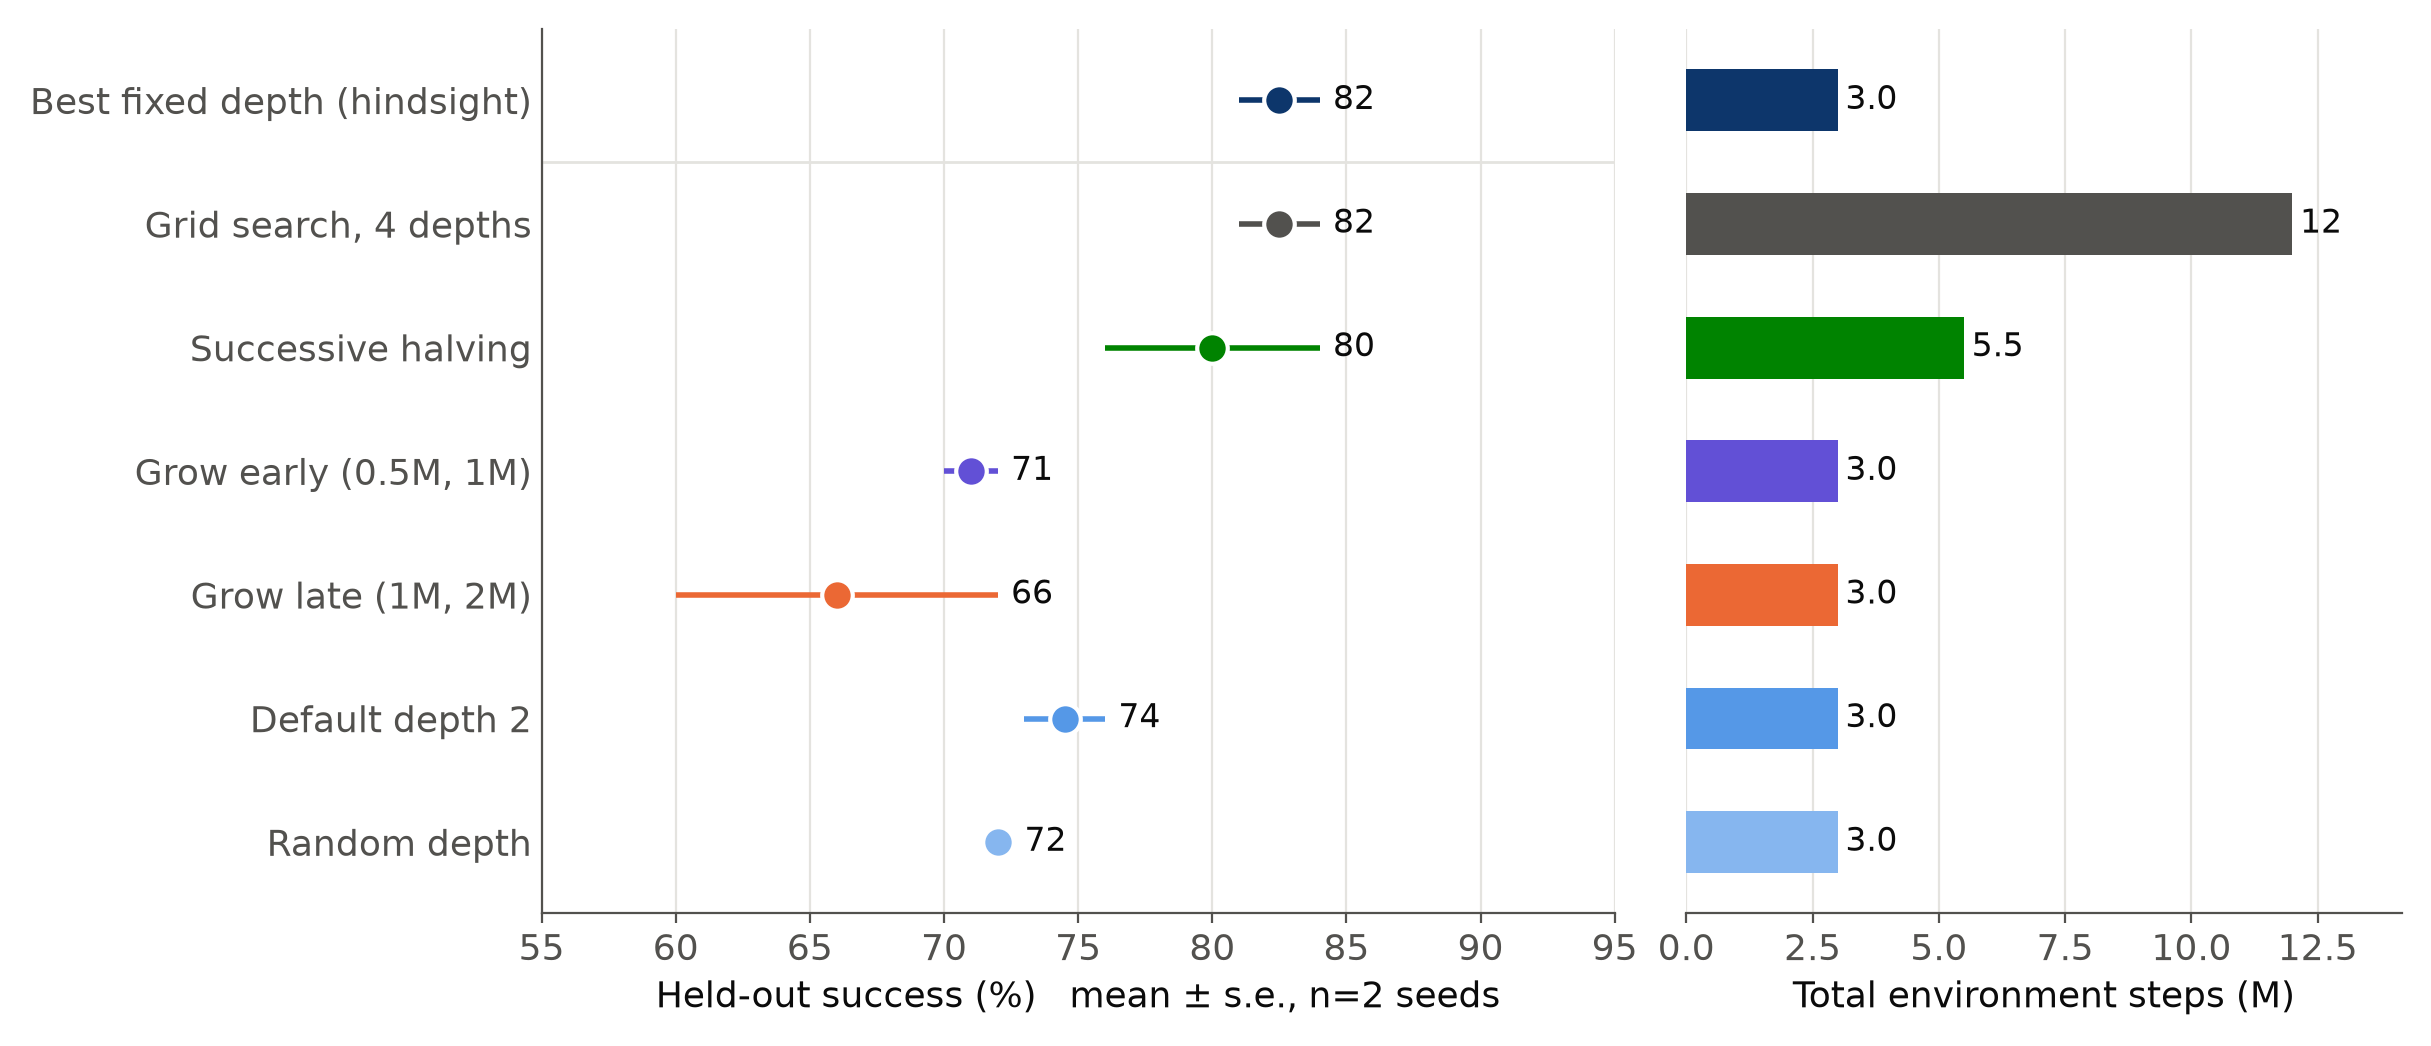
\includegraphics[width=\linewidth]{w128/strategy_panel.png}
    \caption{Strategies at width 128 (two paired seeds).}
    \label{fig:w128}
\end{figure}

\begin{figure}[h]
    \centering
    \begin{subfigure}[t]{0.49\linewidth}
        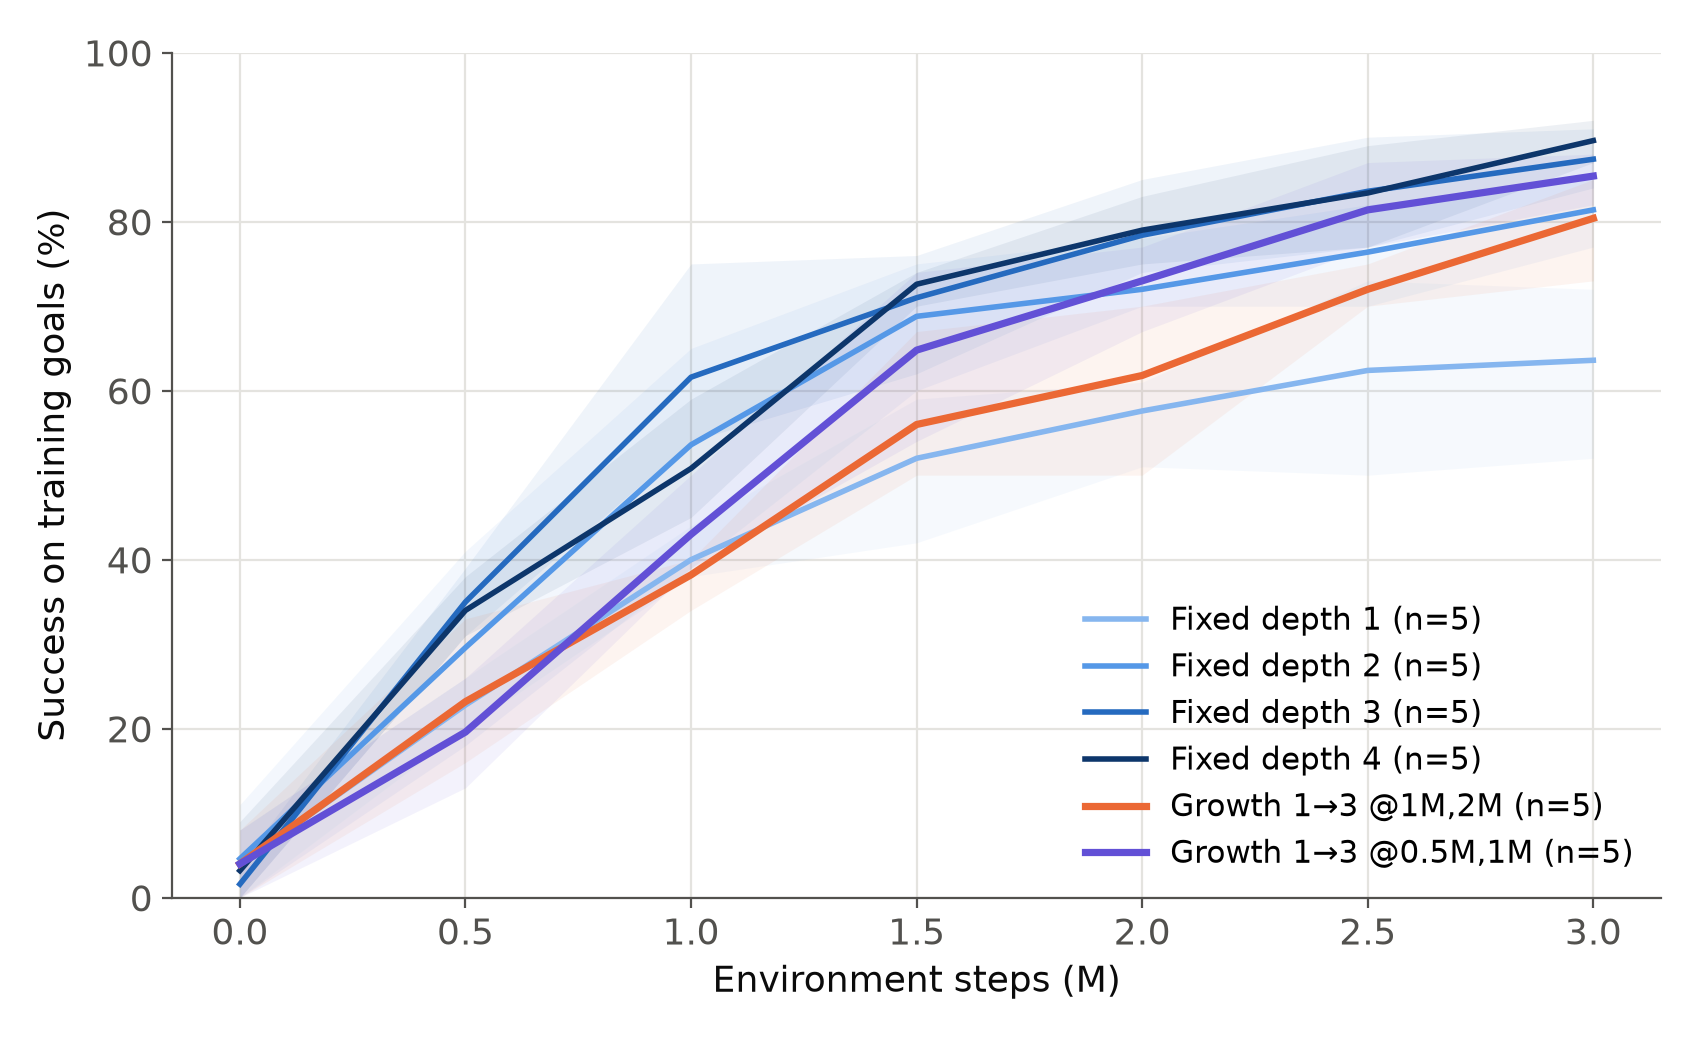
\includegraphics[width=\linewidth]{w400/curves_success_train.png}
        \caption{Training goals}
    \end{subfigure}\hfill
    \begin{subfigure}[t]{0.49\linewidth}
        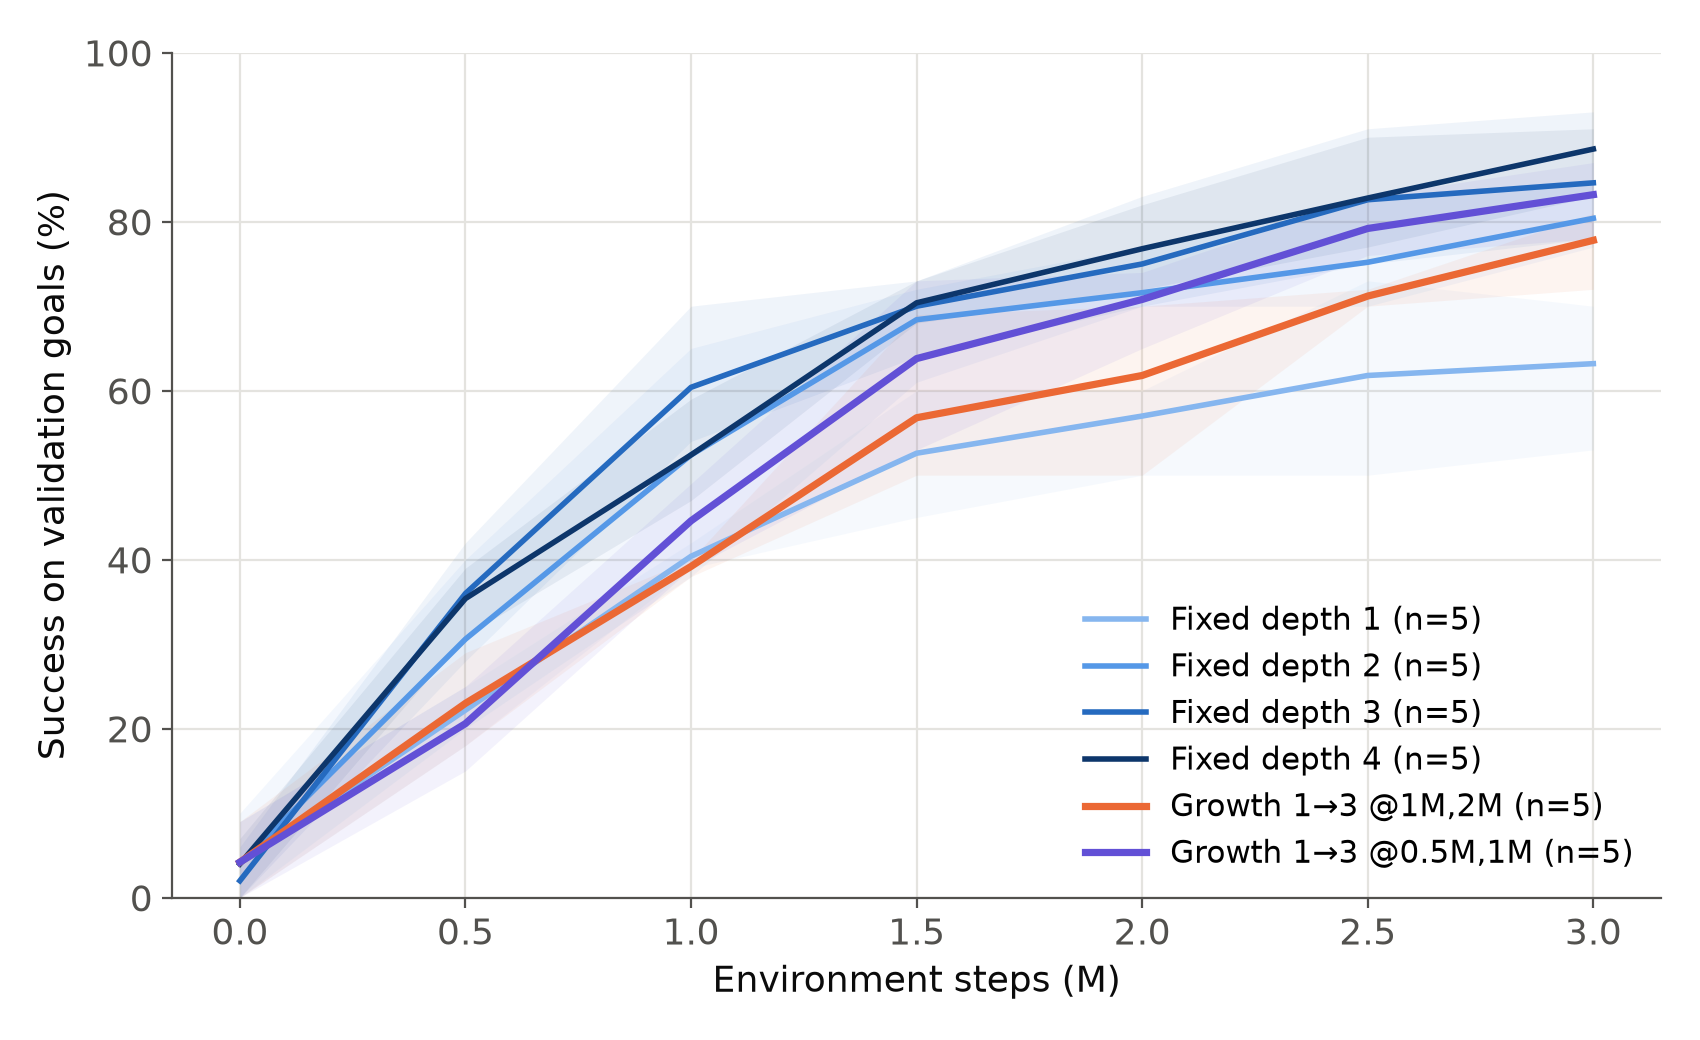
\includegraphics[width=\linewidth]{w400/curves_success_dev.png}
        \caption{Validation goals}
    \end{subfigure}
    \caption{Learning curves on training and validation goals, width 400.}
\end{figure}

\paragraph{Reproducibility.}
The runner (\texttt{sweep\_mt10/}), all per-run logs (\texttt{results/all/}), the aggregation script and every figure are in the project repository.
The runner is an exploratory extension of a frozen timing runner whose source pins it does not preserve; dependency versions are fixed in \texttt{full\_mt10/resolved.lock} (PyTorch 2.8, Meta-World 3.0, MuJoCo 3.7, Tianshou 2.0).
One configuration (depth 4, seed 2) was trained twice after a cloud job appeared to fail and later completed (91\% and 92\%); the aggregation keeps the first by host order (92\%).

\end{document}
